%% Full length research paper template
%% Created by Simon Hengchen and Nilo Pedrazzini for the Journal of Open Humanities Data (https://openhumanitiesdata.metajnl.com)

\documentclass{article}
\usepackage[italian]{babel}
\usepackage[utf8]{inputenc}
\usepackage{johd}
\usepackage{graphicx}
\usepackage{graphics}
\usepackage{listings}
\usepackage{color}

\title{Relazione - Missaggio di un multitraccia con la tecnica mid-side}

\author{Gabriele Acquafredda$^{a}$$^{*}$ \\
    \small $^{a}$2° Anno di Tecnica Del Suono, Primo livello, Dipartimento di Musica Elettronica\\
    \small  Conservatorio di Musica Niccolò Piccinni, Bari, Italia\\
}

\date{Dicembre 2022} 

\begin{document}

\maketitle

\begin{abstract} 
    \noindent La presente relazione vuole studiare i vantaggi e gli svantaggi dell'utilizzo della tecnica mid-side per il missaggio di un brano musicale. L'industria discografica, attualmente, concentra l'utilizzo della tecnica mid-side quasi esclusivamente per le battute finali della produzione dei dischi - vale a dire l'utilizzo di processori quali equalizzatori a fase lineare o compressori nel mastering. L'approccio invece proposto dal seguente esperimento invece è diverso: giungere al master finale passando da un missaggio esclusivamente in mid-side. Il mastering, nella relazione, non è oggetto di studio.
\end{abstract}

\section{Informazioni Preliminari}

\subsection{Il Brano}

Il multitraccia utilizzato per l'esperimento, fa parte dell'archivio delle registrazioni TELEFUNKEN sul sito della Cambridge Music Tecnology. Il brano in questione è Ripe - "4 On The 10" ed è stato registrato live ai "The Lab" della Telefunken.

\subsection{Struttura del Multitraccia e Microfoni Adoperati}

    Il multitraccia presenta i seguenti canali registrati con i relativi microfoni:
    \begin{itemize}
        \item Bass-DI
        \item Chamber - AR70 STEREO
        \item Floor Tom - M82
        \item Hi Hat - M60
        \item Kick In - M82
        \item Kick Out - Cu29
        \item Overhead - AR51 STEREO
        \item Snare Bottom - M80
        \item Snare Top - M60
        \item Tom1 - M81
        \item Chitarra JON - Microfono a Condensatore CU29
        \item Chitarra TORY - Microfono a Condensatore CU29
        \item Chitarra JON - M81
        \item Chitarra TORY . M80sh
        \item Trombone/Horns - M82
        \item Tromba - M81SH
        \item Room - U47 STEREO
        \item Vocal - M80
    \end{itemize}
    Per il missaggio è stato utilizzata la DAW Reaper.
    
\section{Creazione di strumenti ad-hoc per lavorare in M/S}

    \subsection{La matrice M/S}
    Una matrice somma differenza è capace di fare solo calcoli matematici sui segnali: nel nostro caso farà L+R ed L-R, che per definizione sono rispettivamente mid e side. Utilizzare una matrice M/S è la base per lavorare in M/S su tutti i canali. Infatti la adopereremo in tutti i canali per riuscire a convertire tutte le tracce da L/R a M/S. La matrice M/S in Faust si programma nella seguente maniera:
    
    \lstset{frame=tb,
          language=c++,
          aboveskip=5mm,
          belowskip=5mm,
          showstringspaces=false,
          columns=flexible,
          basicstyle={\small\ttfamily},
          numbers=none,
          numberstyle=\tiny\color{blue},
          keywordstyle=\color{red},
          commentstyle=\color{green},
          stringstyle=\color{green},
          breaklines=true,
          breakatwhitespace=true,
          tabsize=3}
          
    \begin{lstlisting}
        import("stdfaust.lib"); //LIBRERIA STANDARD
        nsum = + / sqrt(2);
        ndiff = - / sqrt(2);
        sdmx =  _, _ <: nsum, ndiff; //MAIN
        process = sdmx(_,_);
    \end{lstlisting}

    In questa maniera abbiamo la possibilità di fare dei bilanciamenti M/S semplicemente utilizzando il Panpot di ciascun canale di Reaper.
    Invece per il panning L/R, abbiamo bisogno anche di un altro strumento: un panner mid-side.
    
    \subsection{Mid-Side Panner}
    
    Il codice di Faust adoperato è il seguente:

    \begin{lstlisting}
        import("stdfaust.lib"); 
        
        deg2rad = * (ma.PI/180);
        pp = hslider("Polar Pattern",50,0,100,1)/100 : si.smoo;
        prad = 0 - hslider("Radiants",0,-180,+180,1) : deg2rad : si.smoo;
        
        
        //p figura polare
        //x segnale input
        //rad angolo
        mspan(p,rad,x) = m(p,rad,x) , s(rad,x)
        with{
            m(p,rad,x) = ((1 - p) * x) + (p * x * cos(rad));
            s(rad,x) = x * sin(rad);
        };
        
        vstin = _ , !;
        process = vstin : mspan(pp,prad);
    \end{lstlisting}

    Questo panner ci permette di scegliere la figura polare del mid da adoperare per il panning, variando da Omni (0\%), Cardioide (50\%), Figura a 8 (100\%). Il vantaggio del panner mid side è che lavora non solo sul balance dell'L/R, ma anche sulle fasi di Left e Right, permettendoci quindi di avere una informazione stereofonica più correttamente localizzata nell'immagine stereo dell'intero mix.
    Il secondo slider, invece, ci permette di posizionare precisamente lo strumento nello spazio. Logicamente questo influenza la fase e l'ampiezza in base alla figura polare.
    Come esempio prendiamo un angolo di 225°
    deg2rad ci calcolerà il corrispettivo in radianti che sarà ~3,927.
    Il polar pattern figura a 8 sarà 100, quindi p=1.
    Il mid quindi sarà=(1-1*segnale) + (1*segnale*(-0,71). Essendo la prima parte (che è massima se e solo se p è uguale a 0, vale a dire che stiamo lavorando in omni) nulla, la seconda parte ci darà come risultante un segnale attenuato con un fattore di moltiplicazione dovuto al cos(225°)=~(-0,71) ed invertito di fase.
    Il side avrà: segnale*sen(225°).

    \begin{figure}[H]
        \centering
        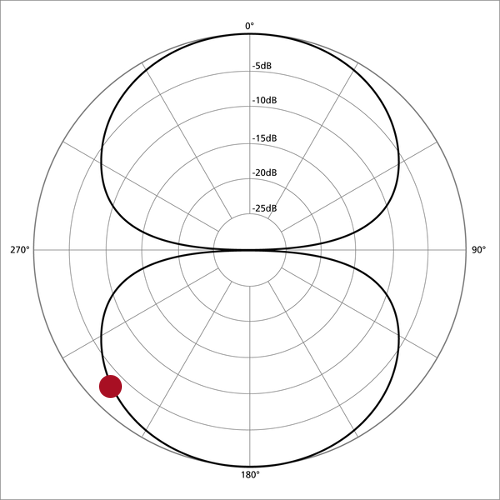
\includegraphics[width=0.5\textwidth]{images/225.png}
         \caption{\label{fig10}Posizione del segnale a 225°}
    \end{figure}

    Se immaginiamo, invece, di avere il segnale esattamente a 90° in una figura a 8: \\
    mid=((1-1*segnale)+(1*segnale*cos(90°)) = 0 - cioè annullamento completo del mid side=segnale*sin(90°) = L e R tra loro in controfase.

\section{Organizzazione della sessione}
    La sessione è stata organizzata tenendo come riferimento delle prassi del missaggio L+R, attraverso delle folder, quindi

    \begin{itemize}
        \item Core ritmico comprendente il drum kit e il Basso
        \item Chitarre
        \item Sezione Brass
        \item Voci
        \item Room e Chamber
    \end{itemize}
    
    Per ciascun canale nativamente stereo, è stato necessario aggiungere la matrice M/S. Per ciascun canale mono, invece, è stato necessario aggiungere l'MSPan.
    Nel master, ovviamente, è necessaria l'operazione di decodifica attraverso un'altra matrice M/S da mettere dopo tutti i VST e prima dell'analizzatore di spettro/loudness ecc.
    
\section{Tecniche M/S Adoperate}    
    \subsection{Routing separato dei plugin}
    Reaper dispone di ampie possibilità di routing per quanto riguarda i plugin nativi e non. Conseguentemente è possibile utilizzare un plugin anche esclusivamente su M o su S.
    Questo può essere molto utile nel caso si voglia fare una compressione differenziata per il mid e per il side, o un'equalizzazione particolare che distingue mid e side.
    Ad esempio: è una mia prassi personale far si che il side sia più scarico nelle frequenze gravi rispetto al mid, in modo da mantenere una certa "centralità" del kick e del basso.
    Questo lo posso fare escludendo dalla matrice di I/O del plugin il mid e facendolo lavorare solo sul side su cui andrò a fare un lowshelf.

    \begin{figure}[H]
        \centering
        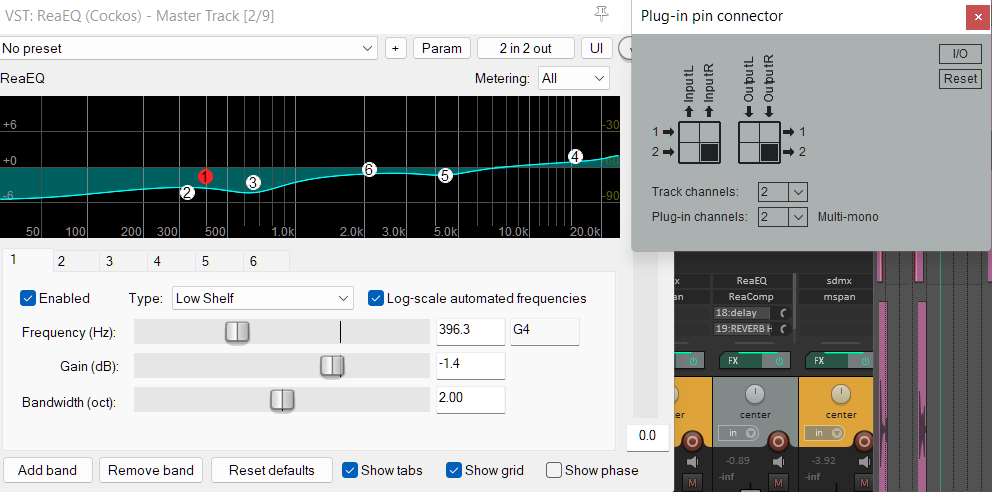
\includegraphics[width=0.8\textwidth]{images/sideeq.png}
         \caption{\label{fig10}Equalizzazione del side sul master}
    \end{figure}

   \subsection{Balance M/S}

   Una volta che nel canale 1 abbiamo il mid, e nel canale 2 abbiamo il side, possiamo utilizzare il pan pot nativo del channel strip di Reaper come un bilanciatore del mid e del side. Questo può essere utile, ad esempio, per bilanciare il mid/side dei canali e "aprirli o chiuderli" verso i lati. Una buona tecnica di missaggio che è stata molto utile per bilanciare la room, il riverbero e la chamber nella sessione. Infatti ciascun canale ha un bilanciamento differente di M/S in modo da avere il proprio spazio in cui "suonare".

   \begin{figure}[H]
        \centering
        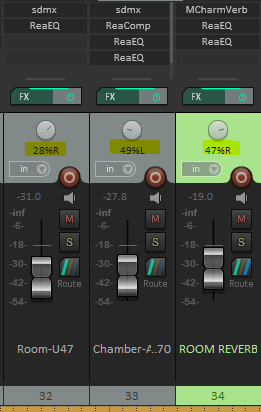
\includegraphics[width=0.35\textwidth]{images/chamberroomrev.png}
         \caption{\label{fig10}Bilanciamento M/S della room, della chamber e del riverbero algoritmico aggiuntivo}
    \end{figure}

    \subsection{Posizionamento degli strumenti nello spazio attraverso l'MSPan}

    Con il nostro strumento MSPan possiamo avere la possibilità di dare una precisa collocazione nello spazio degli strumenti anche servendoci della room stereo fornita nel multitraccia. In questo modo possiamo rendere il risultato finale molto più "naturale" e dare un effetto più live.

\section{Considerazioni Finali: Vantaggi e Svantaggi riscontrati}

    La difficoltà oggettiva nell'utilizzo della tecnica M/S per ciascun canale è quella che i plugin che lavorano esclusivamente in modalità stereo si "scontrano" con un altro tipo di codifica. Ad esempio: un delay ping pong classico come ad esempio quello di Reaper o un H-Delay Waves lavora esclusivamente in stereo. Conseguentemente bisognerebbe scrivere alcuni plugin che lavorino esclusivamente nella modalità M/S, in modo da riuscire ad utilizzare determinati effetti "esclusivi" del L/R anche in M/S.
    Ad esempio possiamo scrivere un delay ping pong verrebbe così codificato:

    \begin{lstlisting}
        declare name "Simple Mid Side Delay";
        declare vendor "G.A.";
        declare author "Gabriele Acquafredda";
        ts = library("12ts.lib");
        
        import("stdfaust.lib");
        import("filters.lib");
        
        
        delay_matrix = hgroup("Delay Matrix",simple_delayL, simple_delayL, simple_delayR, simple_delayR*(-1))
        with {
            del_timeL = hslider("Delay Time L (ms)",0,0,1000,1)*ma.SR/1000;
            del_timeR = hslider("Delay Time R (ms)",0,0,1000,1)*ma.SR/1000;
            
            simple_delayL =  +~(@(2*del_timeL) : *(feedbk));
            simple_delayR = @(del_timeR) : +~(@(2*del_timeR) : *(feedbk));
            
            feedbk = hslider("Feedback %",0,0,110,1)/100;
        };
        
        
        filters = hgroup("Filters", filterlphp, filterlphp)
        with {
            flp = hslider("LoPass Freq",22000,20,22000,1);
            qlp = hslider("LoPass Q",1,1,5,0.05);
        
            fhp = hslider("HiPass Freq",20,20,22000,1);
            qhp = hslider("HiPass Q",1,1,5,0.05);
        
            filterlphp = resonlp(flp,qlp,1) : resonhp(fhp,qhp,1) ;
        };
        
        
        mod_matrix = hgroup("Modulation", modulations, modulations)
        with {
            freq_down = hslider("Downsample Frequency",22000,20,22000,1);
            modulations = ba.downSample(freq_down);
        };
        
        process = _ , _ <: delay_matrix :> mod_matrix : filters;
    \end{lstlisting}

    Questo però può essere un ottimo stimolo per scrivere dei codici che lavorano in maniera personalizzata. In questa versione personale, ad esempio, c'è una sezione dedicata ad HiPass, LoPass e Modulazione, in modo da dare un sound più accattivante al nostro ping pong delay.
    Stessa cosa vale anche per il chorus, il doubler e tutti gli altri tool che lavorano in L/R.
    Il vantaggio principale, invece, è quello di una migliore gestione del panorama stereo. L'utilizzo del panner M/S è molto più naturale rispetto al balance L/R, andando ad evitare automaticamente dei fenomeni di masking e di discordanza di fase. Infatti, una volta posizionati nel panorama stereo, gli strumenti risultano già naturalmente mixati tra di loro, dando la possibilità di intervenire il meno possibile sulla post-produzione, se non per ottenere qualche artefatto particolare altrimenti non ottenibile.
    Un buon compromesso per semplificare il lavoro di missaggio integrando le nuove tecniche adoperate per questo multitraccia, potrebbe essere quello di utilizzare delle tecniche ibride tra L/R e M/S. Se, ad esempio, abbiamo un plugin che lavora in L/R a cui non possiamo assolutamente rinunciare, possiamo provvedere ad effettuare la codifica M/S dopo averlo messo nella nostra catena, in modo da avere una parte della catena del nostro canale che lavora in L/R e una parte in M/S.
    Un altro svantaggio riscontrabile è quello di non avere un metering L/R di ciascun canale, ma solo M/S. Anche questo è raggirabile attraverso la scrittura di un meter L/R che legga segnali M/S.

\subsection{M/S vs. L/R: quale tecnica preferire e perché}

    La risposta è variabile in base al materiale di lavoro. Utilizzare esclusivamente la tecnica M/S può essere complesso quanto controproducente, invece utilizzare esclusivamente la tecnica L/R può essere limitante. "Ibridare" le due tecniche, così come accennato anche sopra, può essere un'ottima soluzione.
    Si è parlato anche del materiale di lavoro in quanto nel missaggio di uno strumento solo o di un'orchestra, la tecnica M/S può superare di gran lunga quella L/R, in modo da fare dei posizionamenti molto precisi e naturali dei microfoni adoperati nella fase di registrazione e restituire un'immagine stereo concorde a quella che è la rappresentazione naturale del posizionamento degli strumenti, evitando artefatti e post-produzioni inutili.
    Per quanto riguarda, invece, la produzione di un brano live, il posizionamento attraverso l'MSPan può essere un'ottima risorsa per dare naturalezza al prodotto finale, piuttosto che adoperare la mera differenza d'ampiezza del panner L/R.
    Nella produzione di un disco in senso prettamente discografico, ponderare le due tecniche è fondamentale ed è attualmente anche una prassi soprattutto nelle battute finali di produzione dei brani di musica pop - vale a dire nel mastering.
    Non esiste una tecnica giusta o sbagliata, ma unire le due tecniche, in linea di massima, serve a sopperire agli svantaggi di una tecnica con i vantaggi dell'altra.
\end{document}